\documentclass{article}
\usepackage{fancyhdr}
\usepackage[german]{babel}
\usepackage{mwe}
\usepackage{amsmath}
\usepackage{graphicx}
\pagestyle{fancy}

\author{Philipp Kiss}

\lhead{Philipp Kiss}
\rhead{Information und Codierung}

\begin{document}
\tableofcontents
\newpage

\section{Logikgatter}
\begin{figure}[h]
		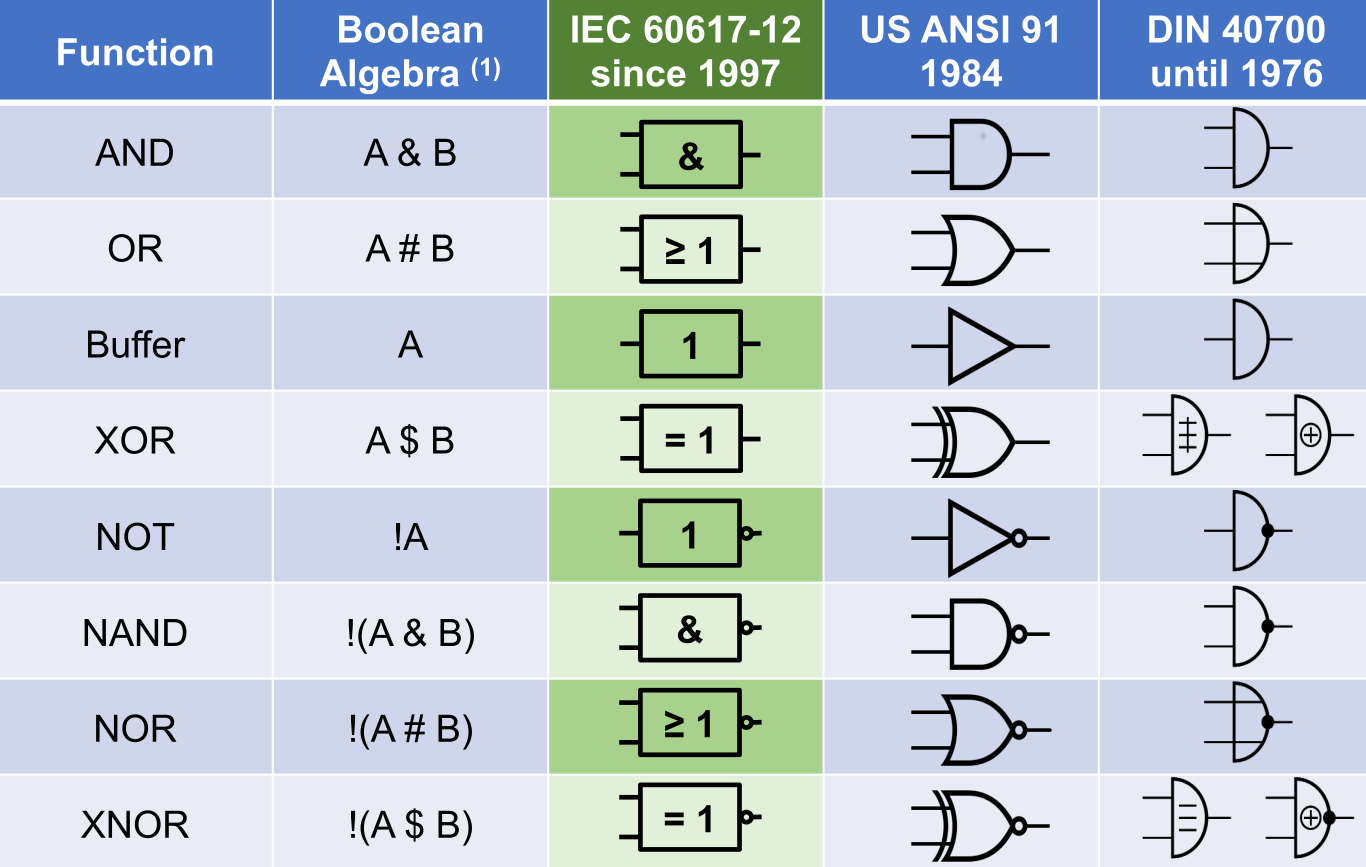
\includegraphics[width=\linewidth]{img/logikgatter.png}
		\caption{verschiedene Logikgatternotationen}
		\label{fig:verschiedene Logikgatternotationen}
\end{figure}
\section{Informationstheorie}
Eine Information ist etwas, was vor seinem Eintreffen noch nicht bekannt war und kann viele Formen annehmen (Ton, Symbol, Text, Wert, ...). Information kann anhand der von ihr beseitigten Unsicherheit gemessen werden. Technisch gesehen ist die kleinste Masseinheit einer Information 1 Bit, sprich eine binäre Entscheidung.
\subsection{Datenquellen}
Eine Datenquelle wird als ``diskret" bezeichnet, wenn sie abzählbare Messwerte liefert. Beispiele dafür sind digitale Sensoren, Ziehung der Lottozahlen, Wetterbericht im Radio. Datenqulle die ``stetig'' sind, liefern nicht abzählbare Messewerte. Beispiele dafür sind jegliche analoge Messewerte (regeln eines Potentiometers, ablesen eines analogen Thermometers).

Zudem kann eine Datenquelle ``memoryless'' sein, wenn die Messwerte statistisch unabhängig voneinander sind.
\subsection{Formeln}
\paragraph{Die Warscheinlichkeit} einer Information wird berechnet, indem man die Vorkommnis der Information durch die gesamten Vorkommnisse teilt. \[
		P(x) = \frac{k(x)}{K} 
\]
\paragraph{Der Informationsgehalt} einer Information wird in Bit angegeben und wird mit \[
		I(x)= \log_{2} \frac{1}{P(x)}
\]
berechnet
\paragraph{Die Entropie} einer Datenquelle bezeichnet den durchschnittlichen Informationsgehalt aller Informationen die diese liefert. Die Masseinheit der Entropie ist $ \frac{\textrm{Bit}}{\textrm{Symbol}} $
\[
		H(x) = \sum_{n=0}^{N-1} P(x_n) \log_{2} \frac{1}{P(x_n)}
\]
\paragraph{Die Mittlere Codelänge} einer Datenquelle beschreibt die durchschnittliche Bitanzahl, die benötigt wird ein Zeichen der Quelle anzuzeigen.
\[
		L = \sum_{n=0}^{N-1} P(x_n) \cdot l_n 
\]
\paragraph{Die Redundanz} einer Datenquelle bestimmt die Ineffizienz der Bitnutzung. \[
		R = L(x) - H(x)
\]

\section{Quellencodierung}
Das Ziel der Kompression ist, redundante und je nach Standard auch irrelevante Informationen zu minimieren um Ressourcen (Zeit, Energie, Bandbreite) zu sparen.
\subsection{Huffman tree}
Der Huffmantree bietet eine garantiert optimale Codierung. Das heisst eine Codierung mit der geringstmöglichen Redundanz. Dafür ordnet man alle Zeichen nach absteigender Probabilität und verbindet die kleinste Probabilität und die nächstgrössere zu einem Ast. Auf diesem addiert man die beiden Probabilitäten und ordnet den Ast neu ein. Diesen Vorgang wiederholt man, bis man an der Wurzel angekommen ist. Zur Überprüfung: die Summe aller Probabilitäten in der Wurzel muss 1 ergeben.
\section{Lauflängenkodierung}
Das Ziel der Lauflängenkodierung ist, Daten möglichst effizient zu speichern. Dabei kann z.B. ``AAAAAABBCCCC'' als ``6A2B4C'' dargestellt werden.
\subsection{LZ77}
Der Lempel-Ziv 77 Algorithmus ist ein verlustfreier, tokenbasierter Textkomprimierungsalgorithmus. Er verwendet einen Vorschaufbuffer und einen Suchbuffer. Dabei werden Muster im Vorschaufbuffer im Suchbuffer gesucht, um festzustellen, ob einen bestimmte Zeichenfolge bereits einmal vorgekommen ist. Dabei wird der beste ``Match'' gesucht. Dieser kann entweder gar nicht gefunden werden (das erste Symbol im Vorschaubuffer wurde noch nie gespeichert) oder einen Treffer von 1 Symbol bis zum gesamten Vorschaubuffer (Falls der komplette Vorschaubuffer so 1:1 bereits abgespeichert worden ist) finden. Ein LZ77-Token besteht aus (Offset|Länge|Symbol). Der Offset besagt, vor wievielen Zeichen der längste Treffer gefunden wurde (0 wenn kein Treffer). Die Länge besagt, wie lang der Treffer war und das Symbol besagt, welches das nächste Symbol nach dem Treffer des Vorschaubuffers war. Die Buffers können variable Längen haben, der Vorschaubuffer muss allerdings 1 Zeichen grösser sein als der Suchbuffer, da ansonsten bei einem Treffer im gesamten Suchbuffer kein weiteres Zeichen aus dem Vorschaubuffer nachgereicht werden könnte.
\begin{figure}[h]
		\begin{center}
		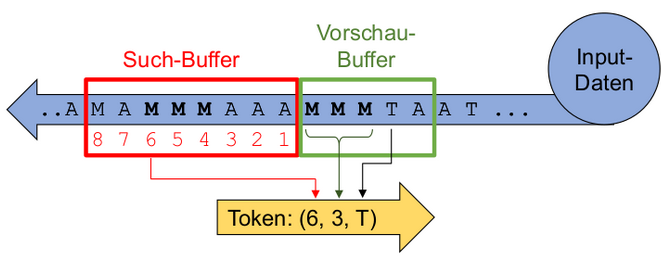
\includegraphics[width=7cm]{img/lz.png}
		\end{center}
		\caption{Illustration des LZ77 Algorithmus}
		\label{fig:Illustration des LZ77 Algorithmus}
\end{figure}
\subsection{LZW}
Der Lempel-Ziv-Welch Algorithmus benutzt im Gegensatz zum LZ77 Algorithmus keine Buffers sondern arbeitet mit einem zur Laufzeit generierten Wörterbuch. Dafür wird jedes Zeichen beim ersten erscheinen mit dem dazugehörigen ASCII-Code (0-255) gespeichert, und als 256-ter Eintrag im Wörterbuch das Zeichen plus das nächstfolgende Zeichen gespeichert. Danach wird immer der beste Treffer gesucht, wobei das Wörterbuch mit jedem weitern Treffer um einen Eintrag wächst und die Einträge immer länger werden, womit bei zunehmender Textlänge und Wortwiederholungsrate die Kompression zunimmt. Um einen LZW-komprimierten Text wieder zu dekodieren wird der Algorithmus ``rückwärts'' ausgeführt. D.h. der erste Token wird aus dem ASCII-Table abgelesen und es wird wieder ein neuer Eintrag an 256-ter Stell angelegt mit dem Zeichen und einem Platzhalter, der mit dem nächsten eingetragenen Zeichen gefüllt wird. So kann das Wörterbuch rekonstruiert werden, was uns erlaubt, es nicht abzuspeichern was noch mehr Speicherplatz spart.
\begin{figure}[h]
		\begin{center}
		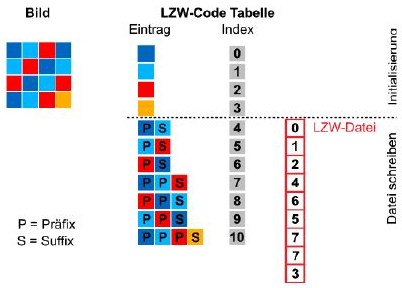
\includegraphics[width=7cm]{img/lzw.png}
		\end{center}
		\caption{Illustration des LZW Algorithmus}
		\label{fig:Illustration des LZW Algorithmus}
\end{figure}
\section{Mediakompression}
\subsection{JPEG}
Das JPEG-Kompressionsverfahren ist ein \textbf{verlustbehafteter} Kompressionsalgorithmus, welcher sich zur komprimierung natürlicher Bilder eignet. Der JPEG-Algorithmus umfasst 7 Schritte.
\subsubsection{Farbraumtransformation}
Unser Auge ist empflindlicher auf Helligkeitsunterschiede als auf Farbunterschiede. Das ermöglicht eine stärkere verlustbehaftete Kompression der Farben bevor wir markante Unterschiede feststellen können. Deshalb trennen wir die 3 Farbelemente aus dem RGB Farbraum auf in eine Helligkeitskomponente, einen Grün-Rot-Wert und einen Grün-Blau-Wert. Das das grüne Farbspektrum bleibt so stäker erhalten, da wir evolutionär bedingt empfindlicher auf Grünabstufungen sind als für andere Farben. Deshalb trennen wir die 3 Farbelemente aus dem RGB Farbraum auf in eine Helligkeitskomponente, einen Grün-Rot-Wert und einen Grün-Blau-Wert. Das das grüne Farbspektrum bleibt so stäker erhalten, da wir evolutionär bedingt empfindlicher auf Grünabstufungen sind als für andere Farben.
Die Y-Komponente entspricht dem Graustufenbild des Ursprungbildes.
\begin{figure}[h!]
		\begin{center}
		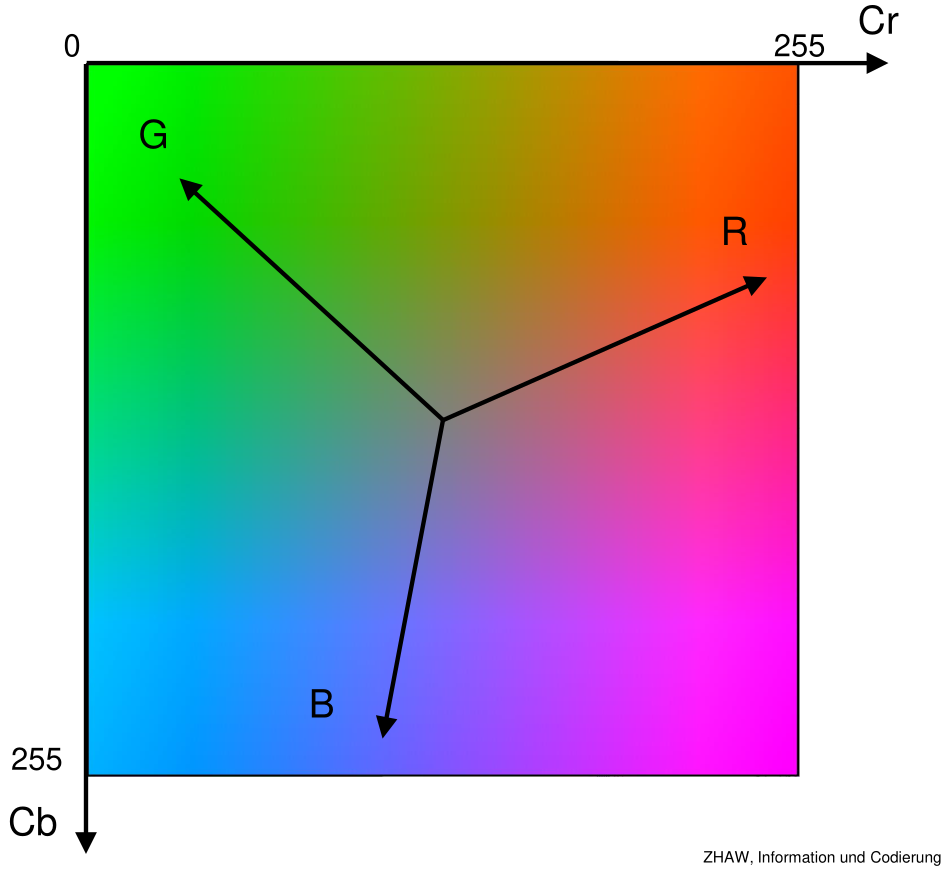
\includegraphics[width=5.5cm]{img/cbcr.png}
		\end{center}
		\caption{Verhältnis Cb zu Cr}
		\label{fig:Verhältnis Cb zu Cr}
\end{figure}
\subsubsection{Chrominanz Downsampling}
Unter dem Chrominanz Downsampling versteht man das Zusammenfassen mehrere Pixel der Farbebenen. Hier werden das erste Mal irrelevante Informationen ``eliminiert''. 
\begin{figure}[h]
		\begin{center}
		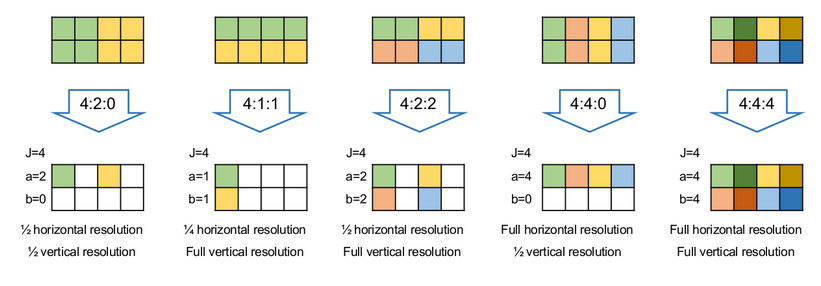
\includegraphics[width=\linewidth]{img/downsampling.png}
		\end{center}
		\caption{Chrominanz Downsampling}
		\label{fig:Chrominanz Downsampling}
\end{figure}
\subsubsection{Pixel-Gruppierung}
Die Idee der nächsten Schritte ist, kleine Pixelgruppierungen möglichst effizient abzuspeichern. Dafür wird das jeder Informationskanal in 8x8 Pixelblöcke aufgeteilt, die dann jeweils gemeinsam komprimiert werden. Falls ein Kanal nicht sauber in 8x8 Pixelblöcke unterteilt werden kann, wird bei den inkompleten Blöcken am Rand entweder die letzte Spalte oder Zeile dupliziert, bis der Block voll ist oder den fehlenden Blöcken wird ein fixer Wert 0 zugewiesen. Beide Optionen führen zu kleinen, kaum spürbaren Artefakten an den Rändern.
\newpage
\subsubsection{Diskrete Cosinustransformation}
Dieser Schritt dient zur Übersetzung der Informationskanäle von Werten von 0-255 zu einer Kombination aus Cosinusfunktionen mit variiernder Frequenz und ist komplett verlustfrei. 
Die Pixelblöcke werden einer nach dem anderen zu einer gewichteten Addition der Cosinusfunktionen übersetzt, da die Koeffizienten weniger Speicherplatz benötigen als die Werte der einzelnen Pixel selbst.

\begin{figure}[h]
    \centering
    \begin{minipage}{0.45\textwidth}
        \centering
        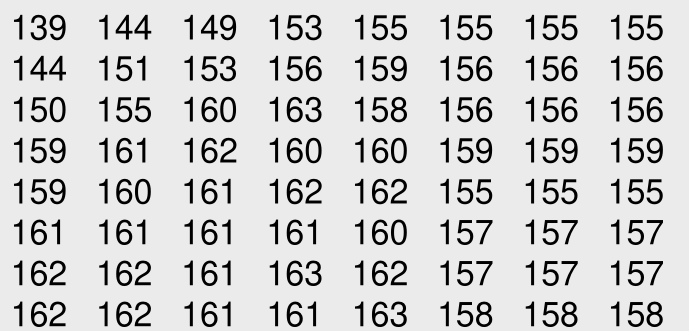
\includegraphics[width=0.9\textwidth]{img/8x8_array.png} 
        \caption{8x8 Pixelarray}
    \end{minipage}\hfill
    \begin{minipage}{0.45\textwidth}
        \centering
        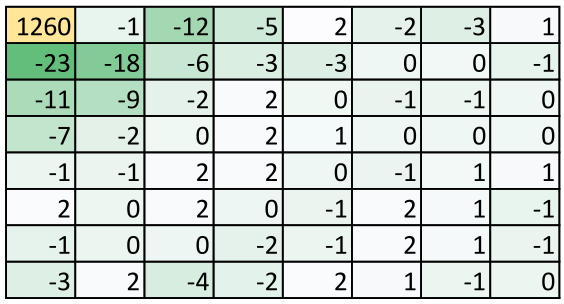
\includegraphics[width=0.9\textwidth]{img/dct_result.png} 
        \caption{8x8 Frequenzarray}
    \end{minipage}
\end{figure}

Es findet also bereits eine verlustfreie Kompression statt. Für die Kompression verwendet man die Forward DCT über dem 2 dimensionalen 8x8-Pixelblock Array und erhält daraus für jeden Pixelblock ein 2 dimensionales Frequenzarray indem die jeweiligen Koeffizienten festgehalten werden. Die Forward DCT sieht wie folgt aus:
$$F_{vu} = \frac{1}{4} C_u C_v \sum_{x=0}^7 \sum_{y=0}^7 B_{yx} \cos \left( \frac{(2x+1)u\pi}{16} \right) \cos \left( \frac{(2y+1)v\pi}{16} \right)$$
\begin{figure}[h]
		\begin{center}
		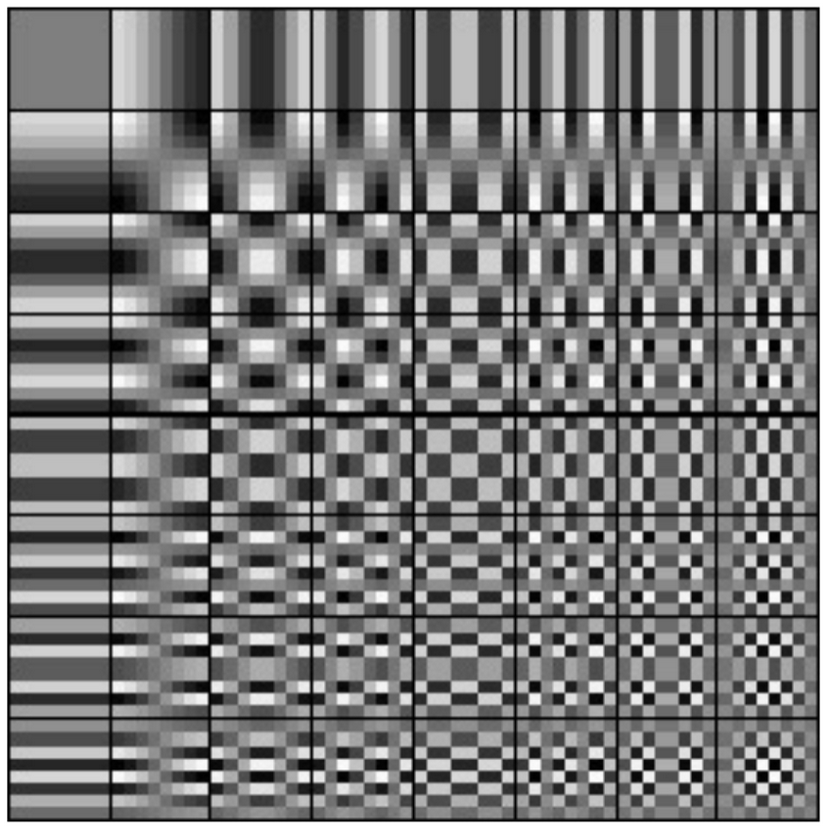
\includegraphics[width=6.5cm]{img/dct.png}
		\end{center}
		\caption{8x8 Cosinusfunktionsmatrix}
		\label{fig:8x8 Cosinusfunktionsmatrix}
\end{figure}
\newpage
\subsubsection{Quantisierung}
Die Quantisierung ist der letzte verlustbehaftete Schritt im ganzen Kompressionsverfahren. Hierfür verwendet man je nach gewünschter Kompression eine tolerantere oder eine aggressivere Quantisierungstabelle. Eine Quantisierungstabelle ist eine Tabelle die analog zu den Pixelblöcken 8x8 Werte beinhaltet, wobei die Werte oben links tiefer sind und gegen unten und gegen rechts höher werden. Indem man alle Werte des Frequenzarrays durch den entsprechenden Quantisierungskoeffizienten teilt und das Resultat auf die nächste ganze Zahl rundet erhält man die Quantisierte Koeffiziententabelle. Dabei gehen feine Unterschiede, die in der ursprünglichen Frequenztabelle unten rechts waren verloren, da sie durch höhere Werte geteilt werden, welche dann auf 0 abgerundet werden. Die massgebenden Frequenzen bleiben dabei besser erhalten.
\begin{figure}[h]
		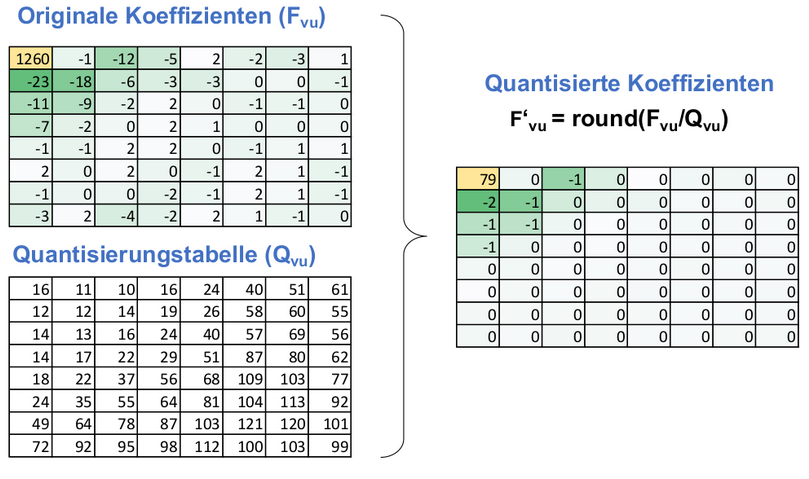
\includegraphics[width=\linewidth]{img/quantisierung.png}
		\caption{Quantisierung}
		\label{fig:Quantisierung}
\end{figure}
\newpage
\subsubsection{Entropy-Coding}
Die Entropiecodierung dient dem effizienten speichern der quantifizierten Koeffizententabelle. Da oben rechts tendenziell höhere Werte sind und unten linke mehr 0 Werte, wird die Matrix in einem Zick-Zack-Muster durchlaufen und diese Tokens mithilfe eines RLE-Verfahrens gespeichert. Das RLE-Verfahren ist im JPEG-Algorithmus nicht genau vorgegeben.
\begin{figure}[h]
		\begin{center}
		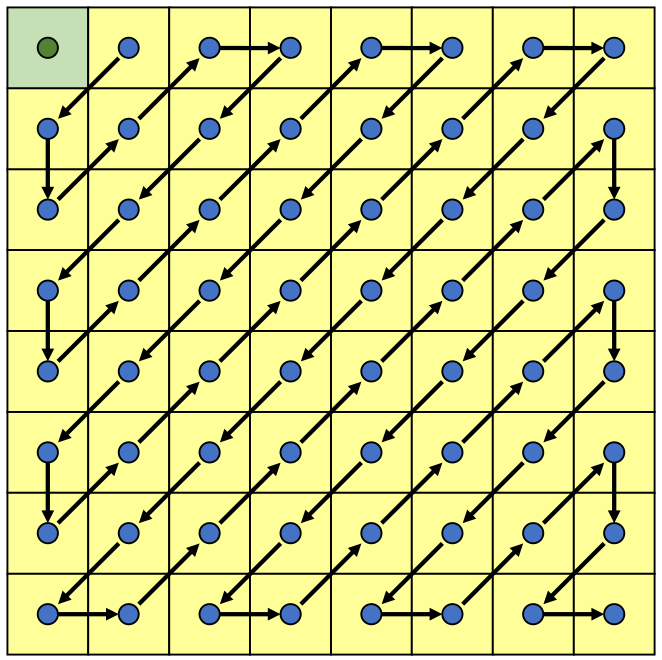
\includegraphics[width=5cm]{img/zigzag.png}
		\end{center}
		\caption{Zick-Zack durchlauf}
		\label{fig:Zick-Zack durchlauf}
\end{figure}
\subsubsection{In Datei verpacken}
Alle Werte die benötigt werden, um das Bild wieder herzustellen werden nun in eine .jpg Datei gespeichert. Das beinhaltet die komprimierte Koeffizentenmatrix sowie die genutzte Quantisierungstabelle und die entsprechenden Anhaltspunkte zum genutzten RLE-Verfahren.

\subsection{Audiokompression}
Schallwellen sind analoge Werte, welche zur Speicherung oder Bearbeitung in digitale Werte umgewandelt werden müssen. Dafür ``tastet'' man die analoge Frequenz ab und arbeitet mit diesen Werten weiter.
\subsubsection{Abtasten}
Das Shannon (oder Shannon-Nyquist Theorem) besagt, dass die Abtastfrequenz für ein Signal mit höchster Frequenzkomponente $\omega$ grösser als $2\omega$ sein muss,um das Signal garantiert verlustfrei abzubilden. Das menschliche Gehör kann Frequenzen bis zu ca. 22kHz verzeichnen, was jedoch von Gehör zu Gehör unterschiedlich ist. Deshalb wird in der Unterhaltung oft mit einer Abtastrate von 44.1kHz oder höher gearbeitet, da wir Frequenzen über 22kHz, die mit einer solchen Abtastrate verloren gehen, sowieso nicht hören würden.

\subsubsection{Quantisierung}
Mit der Quantisierung wird die Amplitude der Abtastpunkte festgehalten. Da das eingehende Signal stetig ist, wir jedoch nur mit diskreten Werten arbeiten können, geht hier unweigerlich Information verloren. Die Auflösung der Quantisierung bestimmt, wie viele Höhenabstufungen für die Amplitude der Frequenz gespeichert werden. Die Werte, welche nicht genau auf einer Höhenabstufung liegen, werden zur nächsten Abstufung auf- beziehungsweise abgerundet.
\begin{figure}[h]
		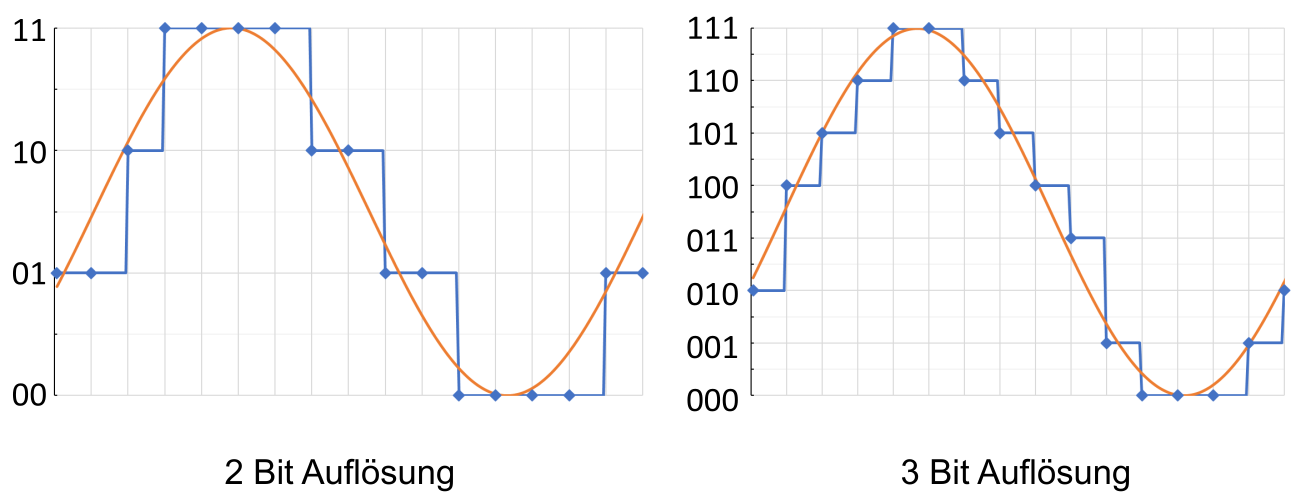
\includegraphics[width=\linewidth]{img/audioQuantisierung.png}
		\caption{Quantisierung eines analogen Signals}
		\label{fig:Quantisierung eines analogen Signals}
\end{figure}
\newline
Bei einer Umwandlung von stetigen zu diskreten Werten entsteht ein Rauschen, so auch bei der Konvertierung von analogen zu digitalen Signalen. Dieses Quantisierungsrauschen ist die Differenz des Rohsignals zu dem digitalen Signal. Daraus folgt, je feiner die diskreten Werte granuliert sind, desto kleiner ist auch das Rauschen. Die Lautstärke des Rauschens beträgt $6\textrm{dB} \cdot \textrm{Anzahl Bit}$
\subsubsection{Pulsecode Modulierung}
Die Pulsecode Modulierung fasst die abgetasteten und quantisierten Menge zusammen, mit dem Ziel, diese möglichst effizient zu speichern/transportieren. Dafür gibt es verschiedene Herangehensweisen. Gemessen wird die Effektivität der Modulierung durch die Bitrate (Bits/Sekunde). Dafür wird die Anzahl Abtastpunkte mit der Quantisierungstiefe multipliziert. Beispiel anhand des europischen Telefonstandards ITU\_T G.711 (A-Law): $$8000\textrm{Hz} \cdot 8\textrm{Bit} = 64 \textrm{KBit/s}$$
Es gibt viele PCM Standards, von denen ein paar hier beschrieben werden.
\paragraph{Linear PCM}
Es wird für jeden Abtastpunkt die Amplitude numerisch festgehalten.
\paragraph{Differential PCM}
Es wird jeweils die Veränderung der Amplitude relativ zum letzten Abtastpunkt numerisch festgehalten.
\paragraph{Adaptive Differential PCM}
Es wird jeweils die Veränderung zur Veränderung der Amplitude relativ zum letzten Abtastpunkt numerisch festgehalten.

\subsubsection{Verlustfreie Audiokompression}
Wave und Flac bieten die Möglichkeit, PCM-Signale verlustfrei abzuspeichern. Wichtig ist dabei, dass nur bei der Speicherung des PCM-Signals keine weitern Information verloren gehen, das gespeicherte digitale PCM-Signal beinhaltet allerdings bereits einen gewissen Verlust gegenüber dem aufgenommenen Analogen Signal. Eine Wave Datei komprimiert das PCM-Signal nicht, wohingegen der Flac-Standard ein Verfahren ähnlich dem LZ-Algorithmus, wodurch eine verlustfreie Kompression möglich ist.
\subsubsection{Verlustbehaftete Audiokompression}
Die Verlustbehaftete Audiokompression 2 Faktoren aus. Zum einen ist unser Gehör nicht gleich empfindlich auf alle Frequenzen. Das erlaubt es uns, nicht/kaum hörbare Töne zu verwerfen und nur die relevanten Frequenzen abzuspeichern.
\begin{figure}[h]
		\begin{center}
		\includegraphics[width=8cm]{img/hörschwelle.png}
		\end{center}
		\caption{menschliche Hörschwelle über dem Frequenzband}
		\label{fig:menschliche Hörschwelle über dem Frequenzband}
\end{figure}
\newline
Weiterer Sparbedarf besteht bei kleinen Amplituden in der Nähe von grösseren Amplituden. Unser Gehör passt sich lauten Schallereignissen an und blendet kurz vor und ein bisschen länger nach einem lauten Ton leisere Töne aus. Je höher die Amplitude eines lauten Ereignisses, desto länger bleibt unser Gehör auf diese Amplitude angepasst. Durch diesen Maskierungseffekt den hohe Amplituden auf kleinere Amplituden ausüben können wir weitere Informationen verwerfen, da diese von unserem Gehör schlechter, wenn überhaupt, wahrgenommen werden können. Dieser Maskierungseffekt wird genutzt, indem das Audiosignal in unterschiedliche Frequenzbänder unterteilt wird, die mit verschiedenen Bittiefen abgetastet werden. Dabei wird die Bittiefe möglichst klein gehalten, wobei das dadurch steigende Quantisierungsrauschen immernoch durch den Maskierungseffekt unter der Höhrschwelle gehalten wird.  
\subsubsection{Schalldruckpegel}
Der Schalldruckpegel ist eine logarithmische Grösse in Dezibel zur Beschreibung der Stärke eines Schallereignises. Berechnet wird er Schalldruckpegel mit folgender Formel: 
$$L = 20 \cdot \log_{2}( \frac{p}{p_0} )$$
, wobei L den Schalldruck in Dezibel repräsentiert, $p$ für den effektiven Schalldruck und $p_0$ den Bezugsschalldruck (die Hörschwelle beträgt $2\cdot 10^{-5}$Pa). Eine Verdopplung des Schalldruckpegels entspricht einer Zunahme von ca. 6dB.
\section{Kanalcodierung}
Da Datenkanäle (=Datenschnittstellen) per se fehlerbehaftet sind, bedarf es einer Codierung der übertragenen Daten, welche den Empfänger erkennen lässt, ob die Übertragung fehlerfrei erfolgte (BEC) oder sogar eine Korrektur der entstandenen Fehler ermöglicht (FEC). Bei allen möglichen Verfahren wird die Rednundanz erhöht, da nicht mehr nur die Daten sondern auch ein Kontrollmechanismus übertragen werden muss. Beispiele für Kanalcodierungen sind positive oder Negative Quittungen, ein erweiterung der Nachricht durch eine Prüfsumme oder simple mehrfache Übertragung. 
\subsection{Bit Error Ratio}
Die Bit Error Ratio, kurz BER, beschreibt die Warscheinlichkeit, dass in einem binären Kanal ein Bit während der Übertragung fälschlicherweise von 1 auf 0 oder von 0 auf 1 gewechselt wird. 
$$\textrm{BER} = \varepsilon = \frac{\textrm{fehlerhafte Bits}}{\textrm{übertragene Bits}} $$
Bei einem symmetrischen Kanal gilt $\varepsilon_{1\to0} = \varepsilon_{0\to 1}$, wohingegen die BER für einen asymmetrischen Kanal ungleich sein können.
\begin{figure}[h]
		\begin{center}
		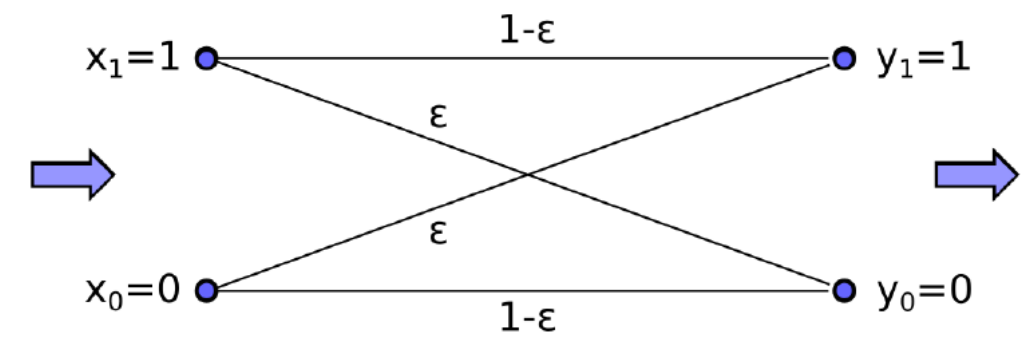
\includegraphics[width=8cm]{img/bsc_error.png}
		\end{center}
		\caption{Fehlerwarscheinlichkeiten eines BSC}
		\label{fig:Fehlerwarscheinlichkeiten eines BSC}
\end{figure}
Die Erfolgswarscheinlichkeit der Übertragung eines Frames $A$ mit einer Anzahl Bit $N$ beträgt $$P_{0,N} = (1-\varepsilon)^{N}$$. Im Umkehrschluss beträgt die Fehlerwarscheinlichkeit $1-(1-\varepsilon)^{N}$.
Die Warscheinlichkeit, dass in einer übertragenen Datensquenz mit $N$ Bits genau $F$ Fehler auftreten beträgt $$P_{F,N} = \binom{N}{F}\cdot \varepsilon^{F}\cdot(1-\varepsilon)^{N-F}$$
Für die Warscheinlichtkeit bis zu einer bestimmten Anzahl Bitfehler $n$, summiert man diesen Term mit $F=0, F=1, ..., F=n$.
\section{Fehlererkennung}
\subsection{Cyclic redundancy check}
Beim CRC-Verfahren, wird das Datenpolynom um die Anzahl stellen eines vordefinieren Generatorpolynoms verschoben, welche zwischenzeitlich mit 0 gefüllt werden. Dieses erweiterte Datenpolynom wird dann durch das Generatorpolynom dividiert, wobei der entstandene Rest der Polynomdivision in die erweiterten Stellen des Datenpolynoms eingefügt wird. Wenn der Empfänger jetzt das entstandene Datenpolynom jetzt durch das Generatorpolynom teilt und etwas anderes als 0 erhält, wurde die Nachricht korrumpiert. Wenn dabei der Rest 0 rauskommt, wurde die Nachricht sehr warscheinlich nicht verändert.
\subsection{Blockcodes}
\section{Fehlerkorrektur}

\end{document}
